%%%%                %%%%
%%%% IMPLEMENTACIÓN %%%%
%%%%                %%%%

\chapter{Implementación}
\label{chap:implemetación}

La implementación está diseñada para recibir peticiones de conversión y generar la salida correspondiente en formato estructurado. El número de ficheros que se pueden tratar en cada ejecución solo está limitado por las capacidades del sistema de ficheros o del SO donde se ejecute. Cada invocación produce una tarea en el sistema, que se gestiona de forma individual. Una vez que se reciben los ficheros para su tratamiento, se crea una ruta específica para ese trabajo y comienza el proceso. En cada etapa se crean nuevos ficheros intermedios que, según se verá más adelante, se mueven a destinos designados para cada paso. Los documentos se tratan a nivel de página individual. El motor encargado de conducir el flujo de información está implementado en lenguaje Bash. Este \emph{engine} se apoya en varias herramientas adicionales, disponibles en cualquier distribución Linux. Por último, se complementa con el generador de código intermedio y los parsers para cada modelo de documento.

% Existen, por tanto, tres partes que se detallarán en las siguientes páginas:

%% \begin{itemize}
%%     \item Un motor o \emph{engine} creado con \emph{scripts} en lenguaje Bash. Su cometido es recepcionar los ficheros y transformarlos paso a paso hasta la obtención de la salida final.
%%     \item Una aplicación Python encargada de generar el lenguaje intermedio que va a ser procesado.
%%     \item Una familia de escáners y parsers desarrollados empleando Flex \cite{estes_flex_2021} y GNU Bison \cite{free_software_foundation_inc_bison_nodate}. Toman como entrada el lenguaje intermedio y lo traducen a un formato estructurado.
%% \end{itemize}

%% Se describen a continuación cada una de ellas.

%% \section{El engine}
%% La herramienta se planteó como un software que pudiera ser capaz de recibir uno o varios ficheros en cada invocación. Una vez recibido, cada entrada debía ser clasificada e identificada para su correcto tratamiento. Dado que la entrada y la salida serían ficheros, resultaba natural utilizar un lenguaje de programación con facilidades para la manipulación de ficheros. Por ser el entorno de operación y desarrollo un sistema GNU/Linux, se optó por emplear el intérprete de \emph{shell} Bash.

%% Por tratarse de un conjunto de \emph{scripts}, este \emph{pipeline} es flexible tanto para añadir nuevos pasos como para quitarlos. La razón para hacerlo de este modo radica en posibilitar la incorporación de nuevas técnicas de procesado de cualquiera área relevante, como el tratamiento de imagen o la extracción de texto. Cada \emph{script} es independiente y puede ser ser activado o desactivado fácilmente.

%% Convenio de nombrado para evitar perder información o mezclar páginas

%% Elaboración de las plantillas: Las plantillas son ficheros en formato JSON. Contienen las coordenadas de la geometría para las regiones de interés.

%% Generación del lenguaje intermedio: el sistema de generación de lenguaje intermedio debía ser necesariamente flexible. Para poder aplicar técnicas distintas. Se optó por utilizar Python, que tiene mucho soporte y una gran colección de librerías disponibles.

%% Detección de subregiones: Se diseñó un algoritmo sencillo pero eficaz para decidir si una región era subregión de otra dada.

%% Aproximación para la identificación de las lineas individuales: Esta aproximación se basó en intentar caracterizar las lineas mediante propiedades sencillas. La aproximación no dio resultado.

%% Mejora de tiempos: Inicialmente se utilizada el tipo de dato Set y sus operaciones para comprobar la inclusión de unas regiones en otras. Esta aproximación, aunque funcional, no resultaba rápida para su ejecución durante el desarrollo. Se realizó una mejora que comprueba las propiedades geométricas en lugar de basarse en lógica de conjuntos.

%% Obtención de información estructurada
%%%% Flex
%%%% Bison

%% Despliegue de la aplicación

%% Cambios para integrarse con la GUI
%%%% Exponiendo las coordenadas 
%%%% Uso de Docker

\section{Estructura física}

Para entender más fácilmente las características de la implementación se describen primero la estructura de directorios que conforman el proyecto. 
La estructura y funcionalidad de los directorios del proyecto es importante para detallar como se trata la entrada. Esta estructura general se puede consultar gráficamente en XXX. La aplicación se compila y distribuye por medio de un \verb|Makefile|. También existe un fichero \verb|Dockerfile| configurado para generar la correspondiente imagen Docker del programa. Los principales directorios utilizados son:

\begin{itemize}
    \item \verb|conf|, empleado para las configuraciones del \emph{engine}, también la configuración de Tesseract y los datos de entrenamiento.
    \item \verb|data| contiene información de los modelos soportados. Principalmente los identificadores utilizados para reconocer los documentos y las plantillas que relacionan las regiones seleccionadas.
    \item \verb|doc| está dedicado a la documentación del proyecto. También contiene todos los ejemplos de ficheros PDF utilizados. Esta memoria, escrita en formato \LaTeX  tiene un repositorio propio.
    \item \verb|engine| tiene como finalidad alojar todos los \emph{scripts} del \emph{engine}.
    \item \verb|input| no está en el repositorio, sino que se crea bajo demanda. Es la ruta base para la entrada de datos utiliza por la aplicación. El nombre puede cambiarse definiendo otro en la configuración del \emph{engine}.
    \item \verb|script| mantiene varios \emph{scripts} auxiliares utilizados principalmente para facilitar las ejecuciones durante el desarrollo.
    \item \verb|tool-gen-language| es la carpeta dedicada a los fuentes de la herramienta de generación de lenguaje intermedio.
    \item Por último, \verb|tool-parser| contiene la aplicación Flex/Bison y los \verb|plugins| que convierten el lenguaje intermedio a la salida JSON.
\end{itemize}

\section{Tratamiento inicial de la entrada}

La herramienta es un software \verb|backend|, no está pensada para que un usuario realice las ejecuciones de la aplicación manualmente. Por ello, y aunque no se desarrolló un API para acompañar la solución, si que se definieron varias características con la finalidad de facilitar la depuración durante el desarrollo y servir de primera aproximación para una futura integración en un sistema con un diseño por capas.

Cada ejecución se lleva a cabo en un directorio propio donde se almacena la entrada, se realiza el tratamiento y se ubica la salida. Además se facilita al programa llamante un identificador que debe utilizar para la recuperación de los resultados. La ruta al directorio que contiene todas las carpetas de todas las ejecuciones el es directorio \verb|input|, mencionado anteriormente.

Para evitar colisiones en las rutas de trabajo durante distintas ejecuciones, se obtiene una marca de tiempo del instante de recepción de la petición y se utiliza directorio como raíz para el nuevo trabajo. Este \emph{timestamp} se obtiene con el comando \verb|date| configurado para generar un entero de tamaño 16 con la hora UTC.

\begin{verbatim}
diego@CompaqCQ57:galiasdoc$ date -u +"%s%6N"
1616623143141490
diego@CompaqCQ57:galiasdoc$
\end{verbatim}

A continuación se presenta la secuencia de pasos que conforman en comienzo de una tarea en el sistema. La primera acción ocurre cuando el invocador del sistema ejecuta el \emph{script} \verb|get-job-id.sh|. Este crea el nuevo directorio para el trabajo y todos los directorios internos. Se devuelve el identificador de trabajo al llamador.

En este momento el llamador debe copiar el fichero de entrada en la ruta \verb|job_id/frontend|. Por último se inicia la ejecución cuando se llama al \emph{script} \verb|run.sh|. El \emph{job} que se debe tratar se indica con el \verb|job_id| pasado como parámetro. Los pasos se pueden seguir visualmente en la figura \ref{fig:inicio-aplicacion}.

A partir de este momento el sistema comienza a trabajar. Cada acción llevada a cabo se indica con un mensaje por la salida estándar de la consola. Cuando finaliza se notifica con otra marca de tiempo del momento final en la ruta \verb|input/job_id/done-<timestamp>|.

\begin{figure}[hp!]
  \centering
  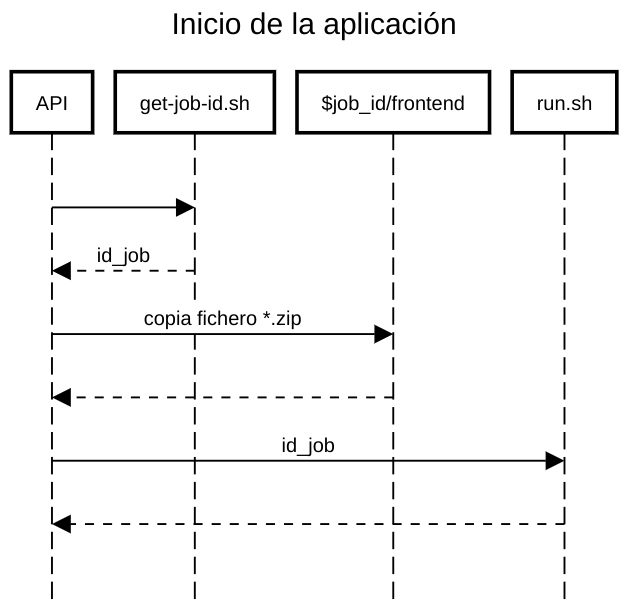
\includegraphics[width=11cm]{imaxes/inicio-aplicacion.png}
  \caption{Secuencia de inicio de la aplicación}
  \label{fig:inicio-aplicacion}
\end{figure}

%% Cambiar diagrama con flecha saliente para indicar que se ejecutan los pasos del engine
%% Cambiar "copia fichero *.zip" por "datos entrada"
%% La linea de finalización debe devolver el evento de finalización

\section{Flujo de información en el \emph{engine}}

Cuando se invoca el \emph{script} \verb|run.sh| se realizan en secuencia todos los pasos que acaban generado la salida en formato estructurado.

\begin{enumerate}
    \item Descompresión de la entrada.
    \item Renombrado seguro de los ficheros.
    \item Extracción de texto con \emph{pdftotext}.
    \item Clasificación de los casos basados en texto y aquellos basados en imagen.
    \item Generación de imágenes para los documentos basados en texto.
    \item Aplicación del OCR para los casos basados en imagen.
    \item Identificación de cada documento.
    \item Generación del lenguaje intermedio.
    \item Invocación del parser necesario.
    \item Publicación de los resultados en el directorio de salida.
\end{enumerate}

Para facilitar la comunicación se asume que la entrada llega  como un fichero comprimido. En este primer paso es necesario extraer los contenidos de dicho fichero. Se realiza además un renombrado de cada uno para evitar errores debidos a caracteres poco amigables con la consola a la hora de componer las rutas.

Una vez los ficheros PDF ya están disponibles se realiza una primera extracción de texto con la herramienta \verb|pdftotext|. El objetivo es realizar la clasificación que separe los ficheros de texto de aquellos cuyas páginas son imágenes.

Cuando \verb|pdftotext| en invocado en un PDF sin texto, genera igualmente un fichero de salida cuyo único contenido es un marcador de fin de página. Por defecto utiliza el caracter \verb|Form Feed| o \verb|0x0D|. Aquellas páginas que dan como resultado únicamente este carácter son movidas al directorio para el tratamiento por imagen, \verb|based-image|.

El siguiente paso consiste en obtener la descripción de las coordenadas de las palabras y las lineas. Para ello \verb|pdftotext| vuelve a ser clave ya que con el flag \verb|-bbox-layout| permite generar un fichero XML que contiene estos datos y también el texto encontrado. Respecto a la calidad del texto hay que tener presente que muchos PDF introducen variaciones en las palabras, típicamente añadiendo espacios entre las letras. Estos problemas son tratados posteriormente.

A continuación se muestra un fragmento de una de estas salidas XML:

\begin{verbatim}
<head>
<title>Factura ES1864857 - OVH</title>
</head>
<body>
<doc>
  <page width="595.000000" height="842.000000">
    <flow>
      <block xMin="1223.064810" yMin="168.431792" xMax="1353.159365" 
          yMax="203.373692">
        <line xMin="1223.064810" yMin="168.431792" xMax="1353.159365" 
        	    yMax="203.373692">
          <word xMin="1223.064810" yMin="168.431792" xMax="1353.159365" 
              yMax="203.373692">Factura:</word>
        </line>
      </block>
    </flow>
  </page>
</doc>
</body>
</html>
\end{verbatim}

%% XXX Explicación de representación en coordenadas

Para facilitar a la aplicación gráfica la visualización de los contenidos detectados surgió la necesidad de proporcionar imágenes de las páginas de los documentos de tipo texto. Esto se realiza invocando a la herramienta \verb|pdftocairo|. 

La siguiente fase se extraen contenidos y coordenadas de las páginas con imágenes. En este caso se utiliza Tesseract. Además del fichero de entrenamiento estándar está disponible otro de mayor tamaño y que resulta más certero con un coste temporal mayor. Para los casos tratados los resultados con la versión estándar fueron suficientemente satisfactorios. Todos los ficheros de entrenamiento de la aplicación están disponibles en la web oficial del proyecto XXX. Existe además la posibilidad de crear ficheros de entrenamiento propios para casos específicos, el proceso también está documentado en la web oficial XXX. La salida de Tesseract que se utiliza no es simplemente el texto reconocido. Al igual que en el caso de las páginas con texto se necesitan las coordenadas de los elementos encontrados. Esto se consigue con el parámetro \verb|tessedit_create_hocr|. La salida en este caso será un fichero en formato HOCR.

%% XXX Imagen del fichero HOCR abierto con alguna aplicación de visualización

Para poder aplicar la plantilla a un fichero correcta a un fichero determinado es necesario realizar un emparejamiento. En este caso se optó por buscar en los documentos datos específicos que no causaran colisión con otros documentos. Dado que los datos disponibles son facturas de empresas, se optó por utilizar los códigos NIF o DNI del emisor en este caso y que por ley son obligatorios en este tipo de documentos XXX. Se creó un registro con estos códigos y se realiza una búsqueda con \verb|grep| sobre los textos extraidos bien con Tesseract bien con \verb|pdftotext|. En los casos tratados esta búsqueda fue lo suficiente robusta.
Cuando un patrón es encontrado, se crea en el directorio donde se está tratando el documento un fichero con el nombre dado al documento en la fase de renombrado y cuyo contenido es el propio identificador encontrado.

\begin{verbatim}
diego@CompaqCQ57:galiasdoc$ ls input/1617643045714091/based-text/2/*id
input/1617643045714091/based-text/2/2.id
diego@CompaqCQ57:galiasdoc$ cat input/1617643045714091/based-text/2/*id
B83834747
\end{verbatim}

Llegados a este punto ya están disponibles toda la información necesaria para construir la salida. Hay dos \emph{scripts} más que se ejecutan. Primero se invoca a la herramienta de generación de lenguaje intermedio y después al parser Bison correspondiente. El último \emph{script} mueve los resultados al directorio de salida del \emph{job}, donde podrán ser recuperados. Además se crea en la raíz del \emph{job} un fichero vacío cuyo nombre es el \emph{timestamp} del momento finalización de de la ejecución.

\section{Generación del lenguaje intermedio}

\subsection{Definiendo regiones con las plantillas}

Las plantillas son documentos JSON que contienen toda la información necesaria para localizar el texto de interés del documento. La creación de las plantillas se ha realizado manualmente. En estas plantillas se definen áreas cuadradas o rectacgulares donde están las palabras que se desea generar en formato estructurado. Se distinguen cuatro tipos de regiones.

La más sencilla es una región de tipo secuencia, esto es, los contenidos se ordenará de izquierda a derecha y de arriba a abajo. Después están las tabla simples que contienen una única columna y múltiples filas o viceversa. El último tipo de región son las tablas de datos con nxm filas y columnas. En el interior de cada subregión el texto se ordena siguiendo el mismo procedimiento que en el caso más básico.

%% Para ampliar: más tipos de informaciones recogidos en las plantillas

\subsection{Flujo principal de los datos}

El cometido principal de la herramienta de generación de código intermedio es transformar el texto extraído en un lenguaje con elementos gramaticales que permitan tratarlo con un parser. A partir de las regiones definidas en las plantillas y las coordenadas de las palabras se hace un filtrado. Se descartan todas las palabras que no encajen en ninguna región, las demás se asocian a la región a la que pertenezcan.

Los elementos principales del programa se detallan a continuación:

Primero se tratan los argumentos de entrada. Especialmente se selecciona XXX ¿qué cosas se seleccionan? XXX
Después se realiza el parse de los datos de entrada. Esto transforma la información de coordenadas y los valores de las palabras en estructuras en memoria. Datos que ambos orígenes de datos comparten el formato HTML, es posible utilizar el parser por defecto que proporciona Python, la clase \verb|HTMLParser|, con la finalidad de extraer las lineas y palabras proporcionadas. Se crearon dos clases que especializan la anterior, \verb|xmlTMLParser| y \verb|hocrHTMLParser| para las particularidades de cada tipo de origen.

En la aplicación existen tres conceptos distintos de lo que es una linea. La idea más inmediata de una linea es aquella que se aprecia visualmente sobre un documento. Estas son las lineas que querríamos que el sistema identificara como tales. XXX extender concepto de linea con las otras dos ideas. Creo recordar: la linea área que encaja dentro de una columnas, pero no se extiende a otras. XXX. Un problema encontrado en esa asignación de palabras a lineas es que hay casos donde una linea abarca más de una columnas. Para generar correctamente el lenguaje, cada palabra debe pertenecer a una única linea y la linea debe pertenecer a una única columna. Se realiza por tanto un troceado de las lineas excesivamente extensas. Se fraccionan y se asignan a las regiones que les corresponden.

En este punto ya se ha preparado la información para poder llevar a cabo el tratamiento. Se crea en un objeto tipo diccionario que contiene todos los datos conocidos hasta ahora:

\begin{itemize}
	\item Las lineas,
	\item las palabras,
	\item las regiones definidas en las plantillas,
	\item el número de página actual,
	\item el número de páginas que contiene el documento completo,
	\item la ruta a la imagen de la página actual.
\end{itemize}

La penúltima fase asigna contenidos a las regiones definidas en las plantillas y por último se escriben todos los resultados a disco.

\subsection{Tratamiento de las lineas y las regiones}

El objetivo principal en esta fase es asociar a cada región las lineas que le corresponden. Primero se realiza una clasificación de las regiones según apliquen a una única página, por ejemplo la primera o la última; a múltiples páginas o a todas las páginas del documento. Lo que se hace es escoger las regiones que aplican a la página actual atendiendo al número de página que tiene y su posición dentro del documento. Además de los casos básicos mencionados anteriormente, para el correcto tratamiento fue necesario implementar comportamientos para las siguientes categorías: 

\begin{itemize}
	\item R1: una región formada por una columna de cabeceras a la izquierda
	\item R2: región con cabecera en la fila superior
	\item R3: región básica con contenidos secuenciales. Se trata como una celda única.
	\item T1: es una tabla bidimensional donde la primera fila contiene la cabecera y tienen múltiples columnas.
	\item T2: similar al caso anterior pero los límites entre las filas de la tabla se calculan por medio de la transformada de Hough.
	\item T2_T2: configuración de dos regiones T2 consecutivas.
	\item T2_T2_R1: región especial formada por una región T2_T2 seguida de una región R1.
\end{itemize}

%% Adentrarse en cómo seleccionan las regiones las lineas que les corresponden.

%% Mostrar tipos de regiones en el apéndice

%% ¿Por qué fue necesario crear las regiones contiguas. Por el documento tipo \emph{papel continuo}. Detallar.

%% Uso de la transformada de Hough para definición de las filas.

\subsection{Creación del lenguaje intermedio}

Por último los contendidos de cada región, se escriben a la ruta de salida. Existe un método para cada tipo de región. Las regiones dobles utilizadas en la fase anterior no se utilizan aquí y solo se trabaja con R1, R2, R3, T1 y T2.

\section{Salida en lenguaje estructurado}
